%%%%%%%%%%%%%%%%%%%%%%%%%%%%%%%%%%%%%%%%%%%%%%%%%%%%%%%%%%%%%%%%%%%%%%%%%%%%%%%%%%%%%%%%%%
\section{Results}

%%%%%%%%%%%%%%% Parameters %%%%%%%%%%%%%%%
% n_data = 20 - n_data in x and y: n_tot = 20*20
% test_size = 0.2
% noise = 0.2 - aptitude of normal distributed noise    
% data_dim = 2

%%%%%%%%%%%%%%% Part b %%%%%%%%%%%%%%%
% * Evaluate MSE up to 5.th order fro OLS. 
% * and R2 score
% * blot parameters beta
% * Your code has to include a scaling/centering:
%   XXX: not included, data is already scaled in intervall [-1, 1]

\begin{figure}
     \centering
     \begin{subfigure}[b]{0.5\textwidth}
         \centering
         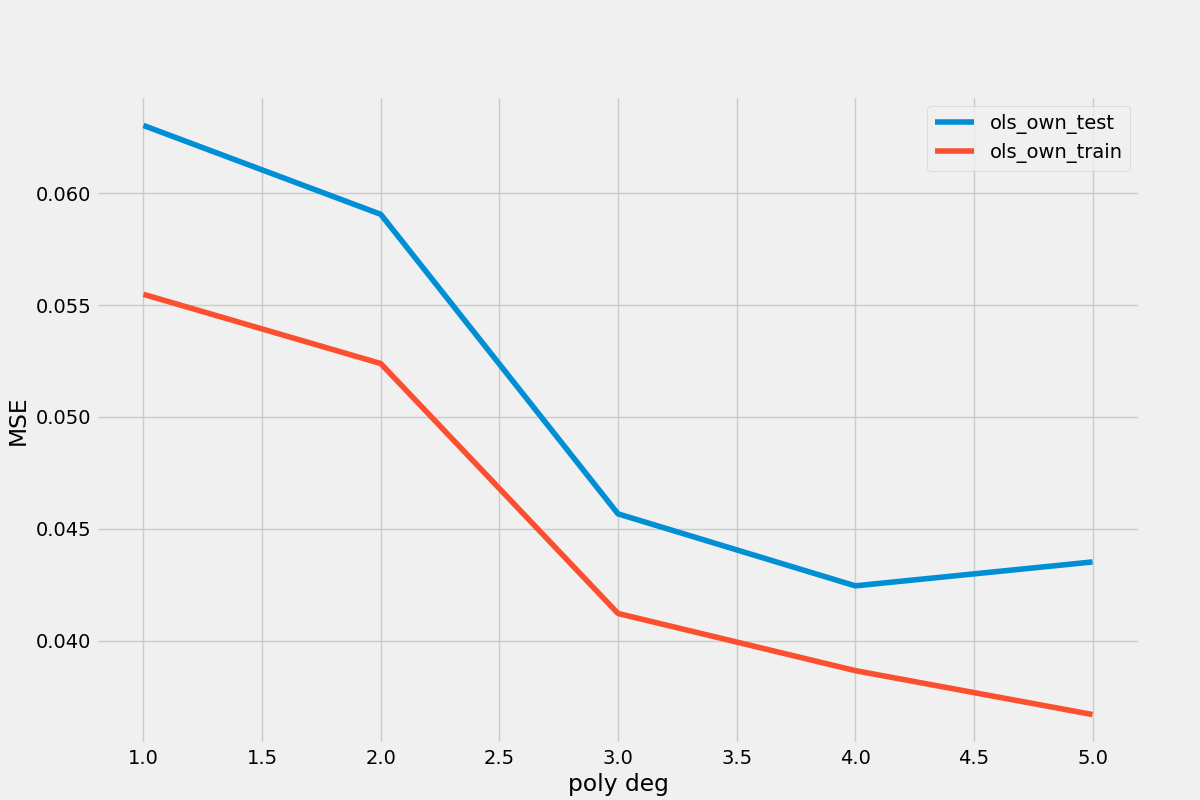
\includegraphics[width=\textwidth]{Figures/b_mse.png}
     \end{subfigure}%
     \hfill
     \begin{subfigure}[b]{0.5\textwidth}
         \centering
         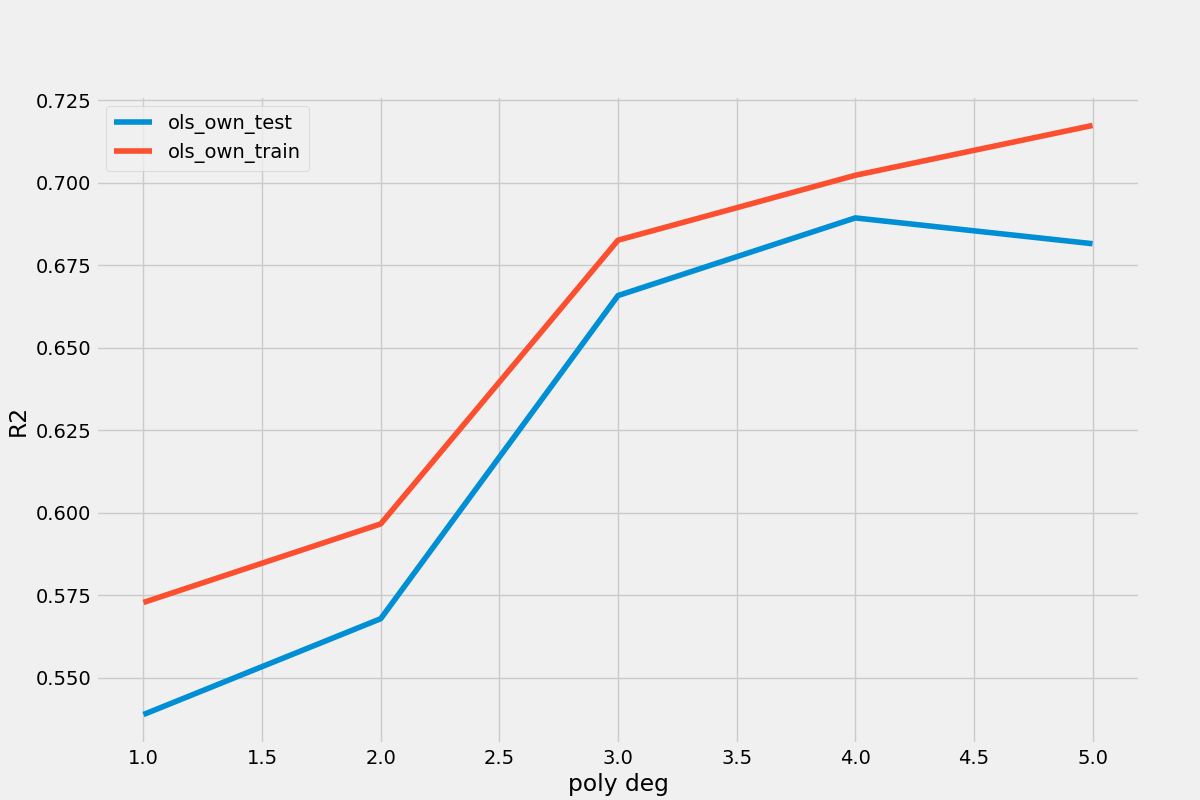
\includegraphics[width=\textwidth]{Figures/b_r2.png}
     \end{subfigure}
        \caption{Mean squared error and score function for the Ordinary Least Squares (OLS) method on the Franke function with N=????? for training and test data with a test/train split of 0.2}
        \label{fig:mse_and_score_franke}
\end{figure}

In figure \ref{fig:mse_and_score_franke} we see the mean squared error and score on the Franke function for a polynomial up to degree five. If our predictors represent different scales, then it is important to standardize the design matrix. And as the x and y data is on the same interval $[0, 1]$ we do not need to scale the data. We see from the figure that we get a big decrease in MSE and big increase in $R^2$ for a polynomial degree up to five. For degree five we do not see much change. 

%\begin{figure}[H]
%    \centering
%    \caption{Mean square error as function of polynomial degree for }
%    \label{fig:ols_franke}
%    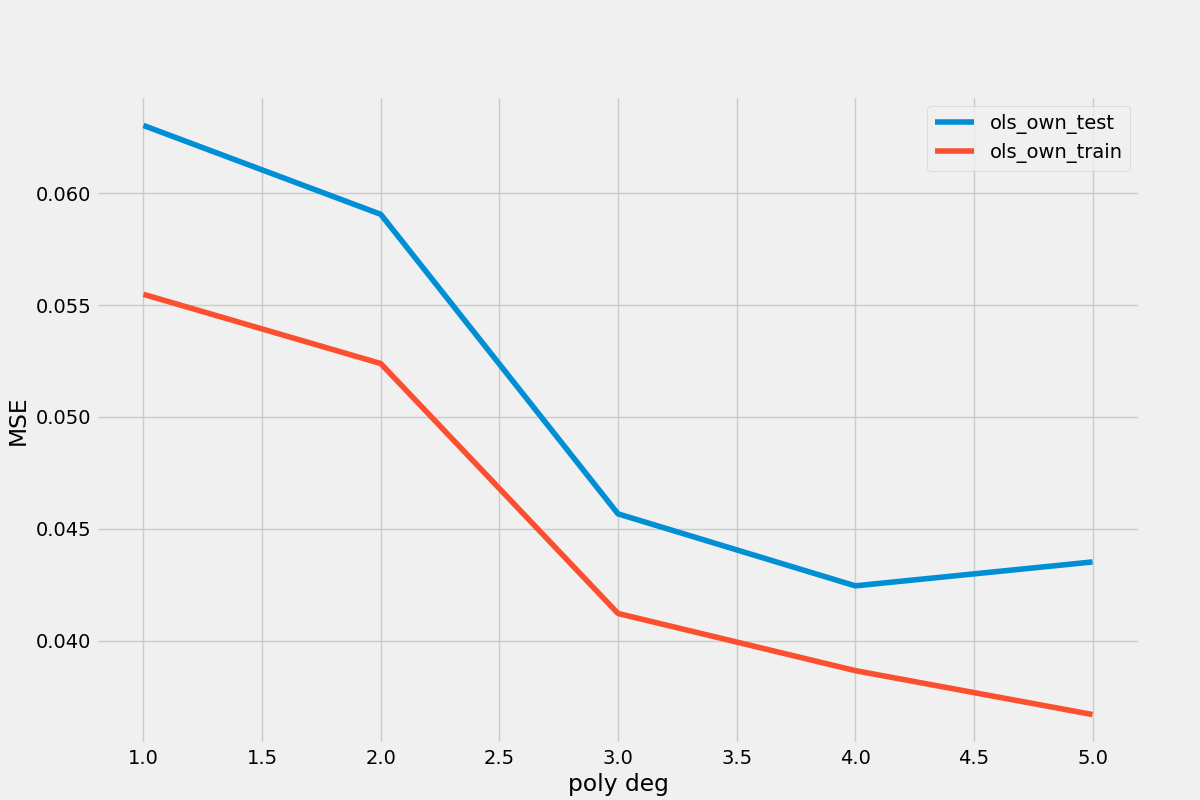
\includegraphics[width=0.8\textwidth]{Figures/b_mse.png}
%\end{figure}

%\begin{figure}[H]
%    \centering
%    \caption{}
%    \label{fig:score_franke}
%    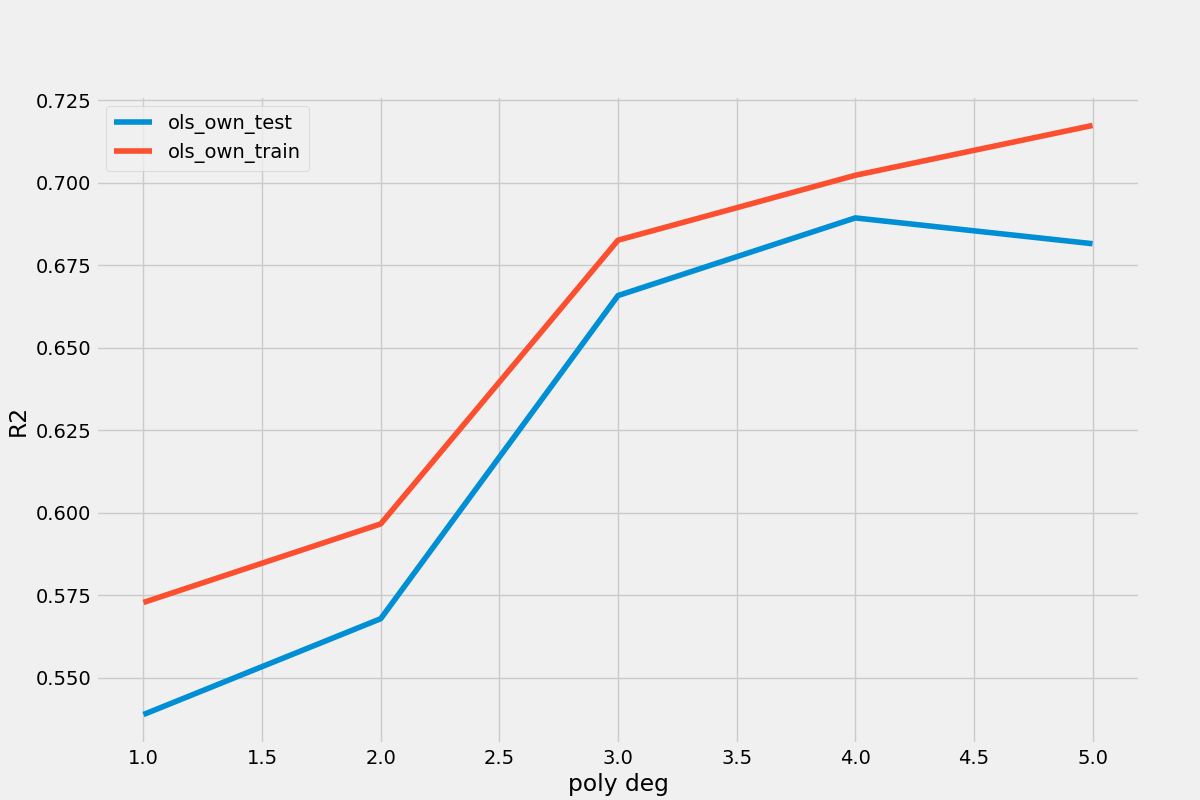
\includegraphics[width=0.8\textwidth]{Figures/b_r2.png}
%\end{figure}

% TODO: error bars
\begin{figure}[H]
    \centering
    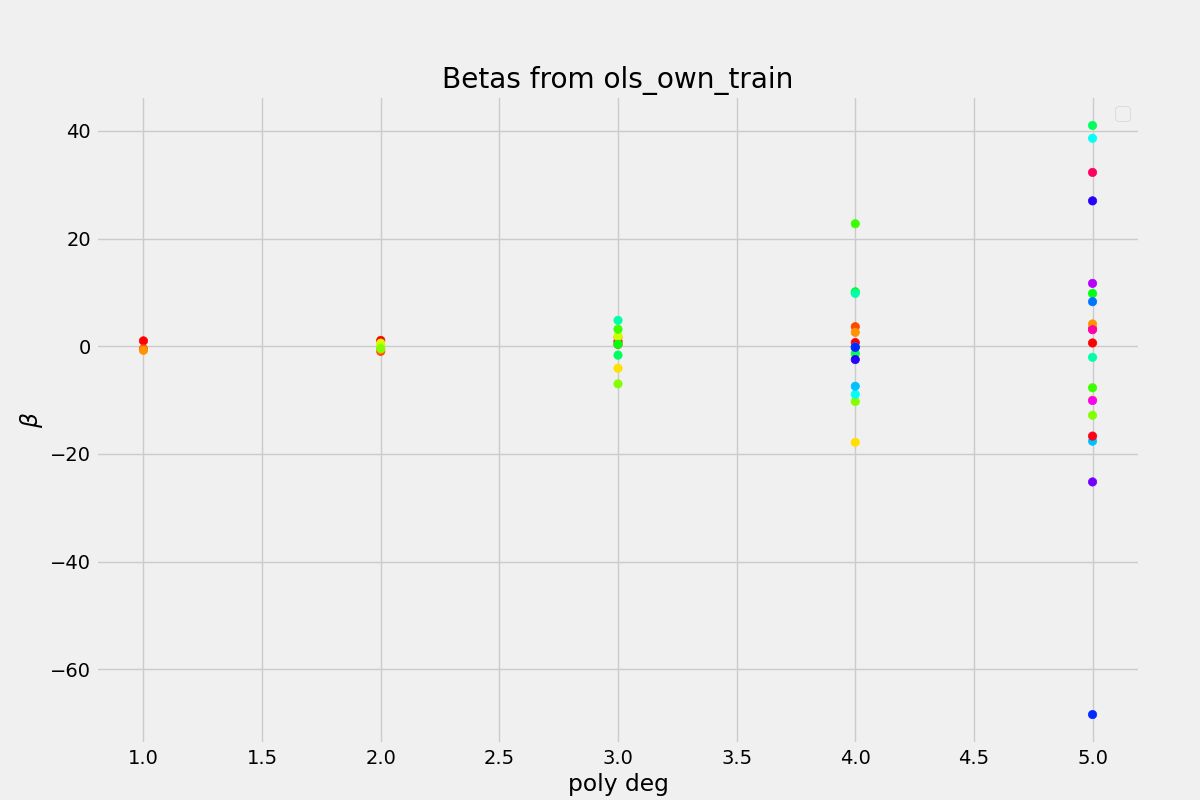
\includegraphics[width=0.8\textwidth]{Figures/b_beta.png}
    \label{fig:beta_plot}
    \caption{$\beta$-parameters of the OLS model on the Franke function for N=????. Ment to illustrate variation in $\beta_i$ as polynomial degree increases.}
\end{figure}

In figure \ref{fig:beta_plot} we see for each polynomial degree the beta parameters $\beta_i$ as a dot in the plot. This is for the OLS model on the Franke function. We see that as the polynomial degree increases, the $\beta$ values deviate more and more from zero. This can be a result of overfitting since we do not have any regularization parameter on the OLS model.

%For bootstrap: should consider plotting a histogram of the estimators beta_hat^* as this should resemble a pdf. 

%%%%%%%%%%%%%%% Part c  %%%%%%%%%%%%%%%
% * Explain bias, variance, mse terms (theory) and interpretation 
% * Bias variance analysis on franke function
% * discuss in bias variance trade-off in terms of:
%   * model complexity
%   * number of data points
%   * training and test data


\begin{figure}[H]
    \centering
    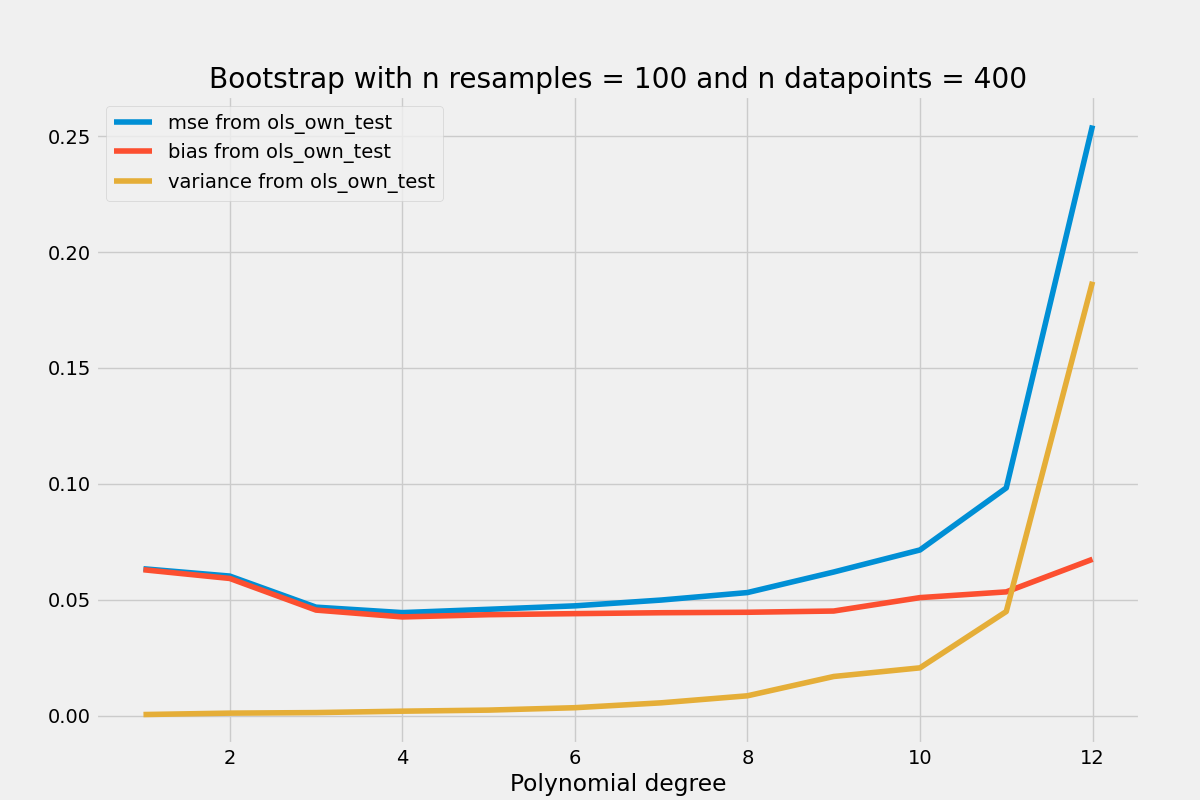
\includegraphics[width=0.8\textwidth]{Figures/c_bootstrap_ols_n_data_400.png}
    
\end{figure}


\begin{figure}[H]
    \centering
    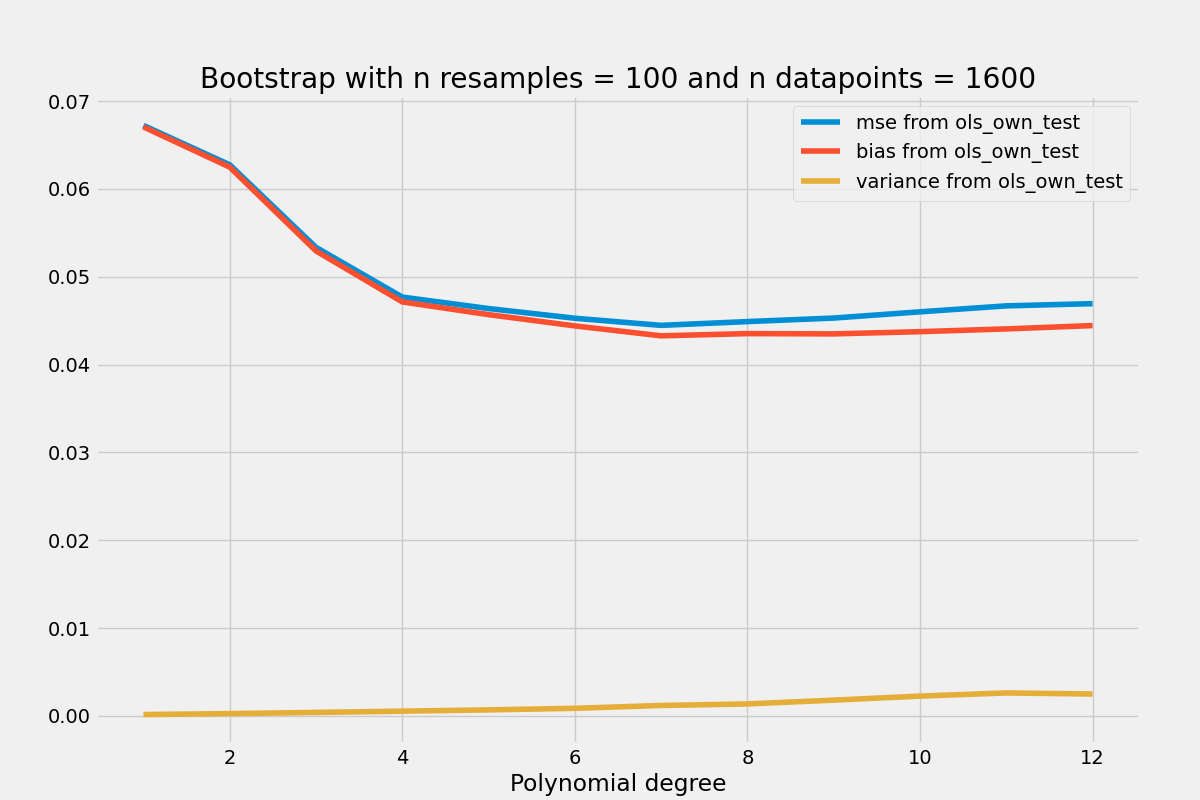
\includegraphics[width=0.8\textwidth]{Figures/c_bootstrap_ols_n_data_1600.png}
\end{figure}

% XXX: Is this expected behaviour?
\begin{figure}[H]
    \centering
    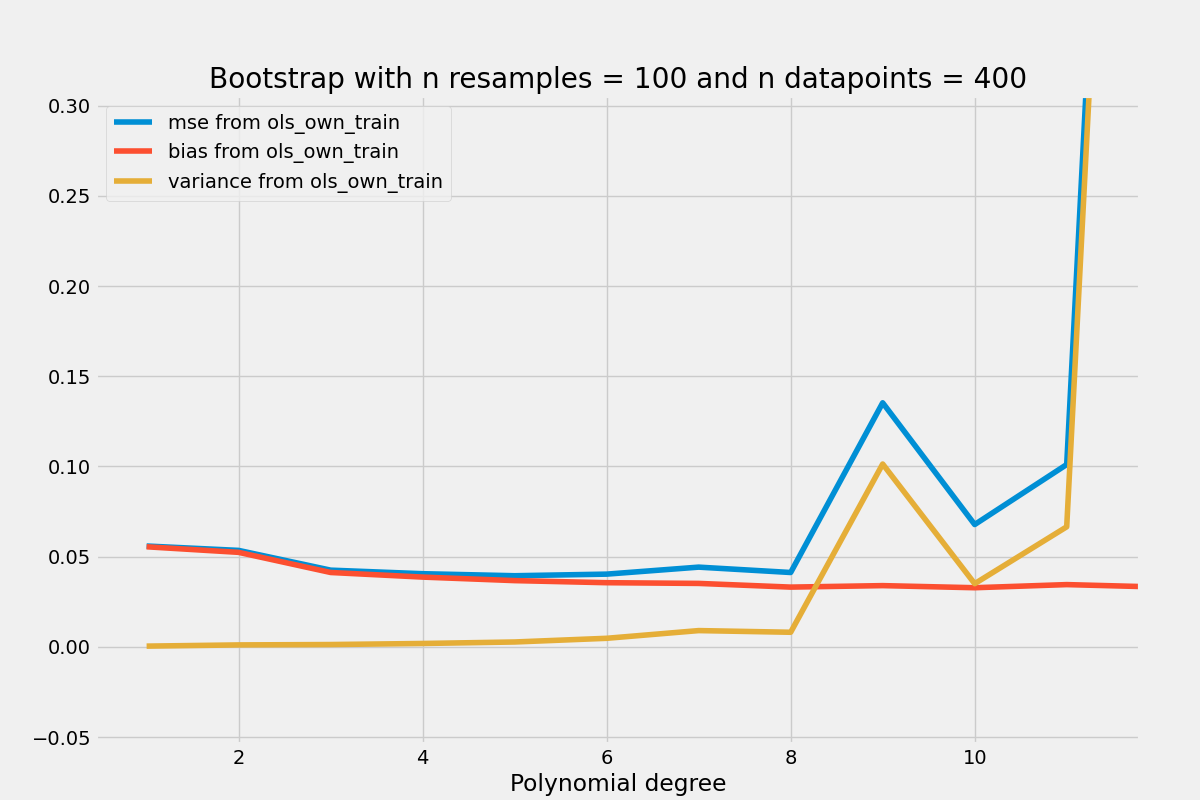
\includegraphics[width=0.8\textwidth]{Figures/c_bootstrap_ols_n_data_400_train_data.png}
\end{figure}

%%%%%%%%%%%%%%% Part d %%%%%%%%%%%%%%%
% Use k-fold and evaluate MEE on test data
% compare with bootstrap
% compare with sklearn

\begin{figure}[H]
    \centering
    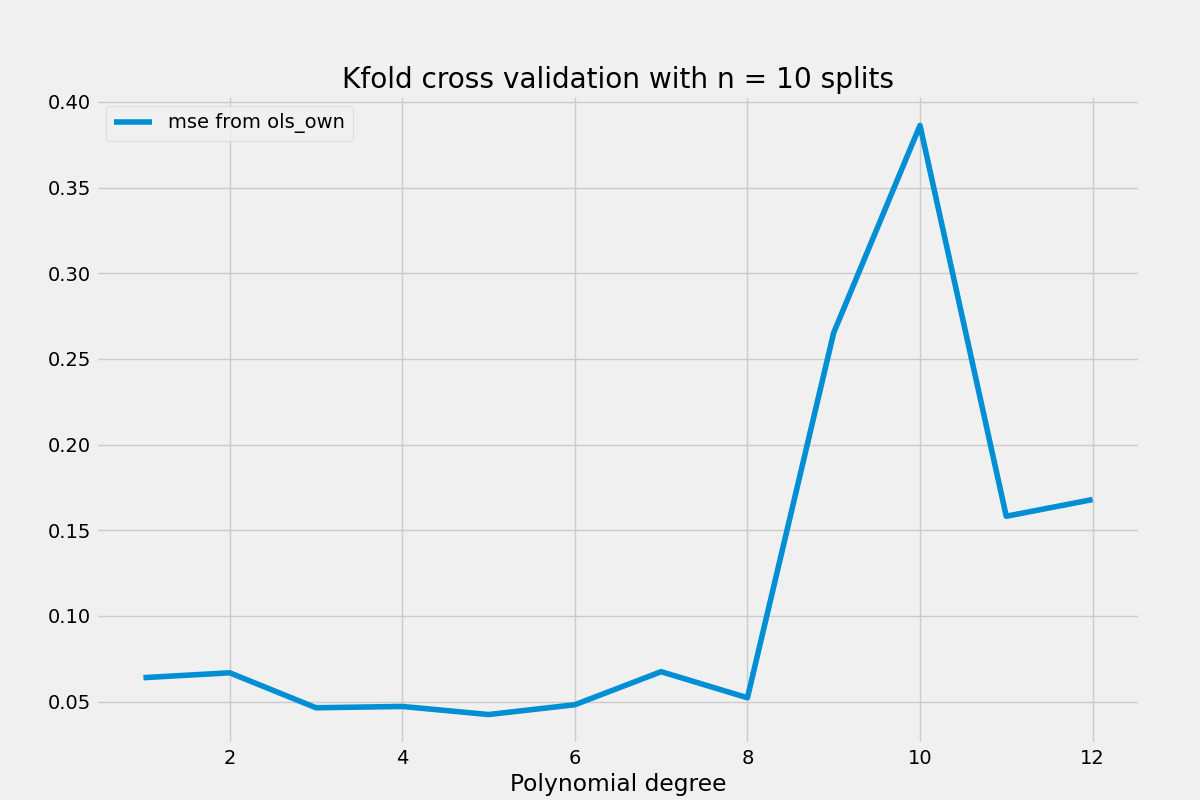
\includegraphics[width=0.8\textwidth]{Figures/d_kfold_ols_n_10.png}
\end{figure}

%%%%%%%%%%%%%%% Part e %%%%%%%%%%%%%%%
% * bootstrap analysis for ridge as in part c
% * and cross validation as in part d 
% * Compare results to those obtained in part b-d
% * study bias variance trade off for different values of lambda 

The minimum MSE from Ridge regression was found for polynomial degree of 6 with
the hyper parameter, $\lambda = 0.001$
\begin{figure}[H]
    \centering
    \caption{ridge}  
    \label{fig:e_ridge} 
    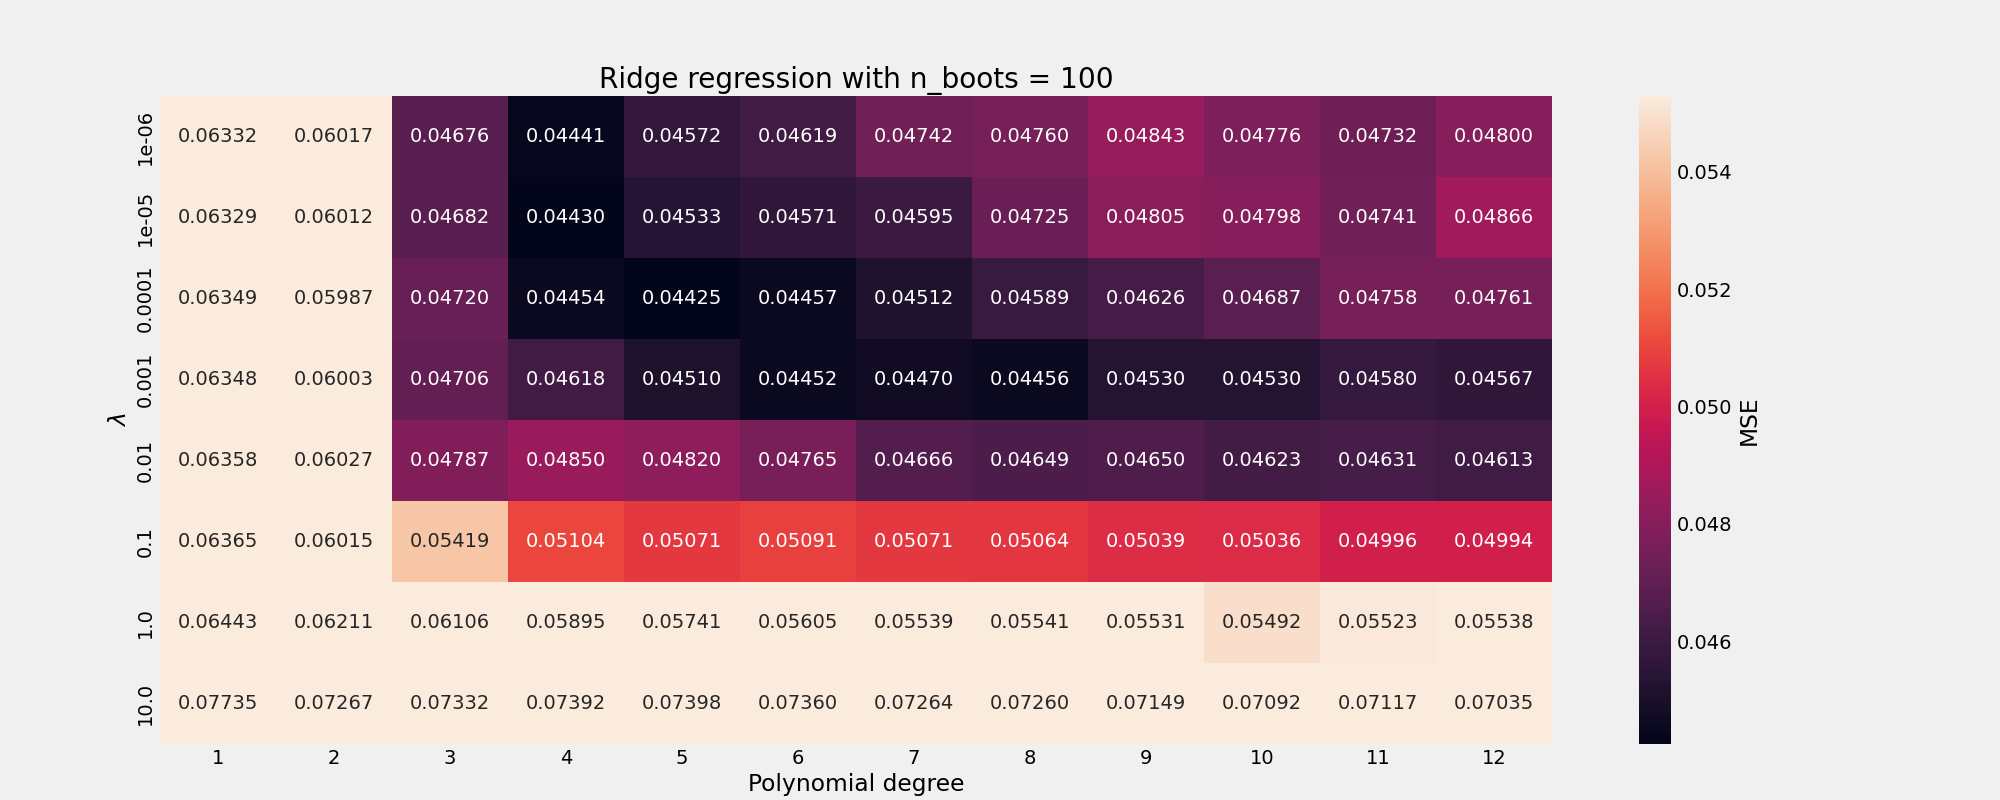
\includegraphics[width=1\textwidth]{Figures/e_ridge_n_boots_100.png}
\end{figure}

\begin{figure}[H]
    \centering
    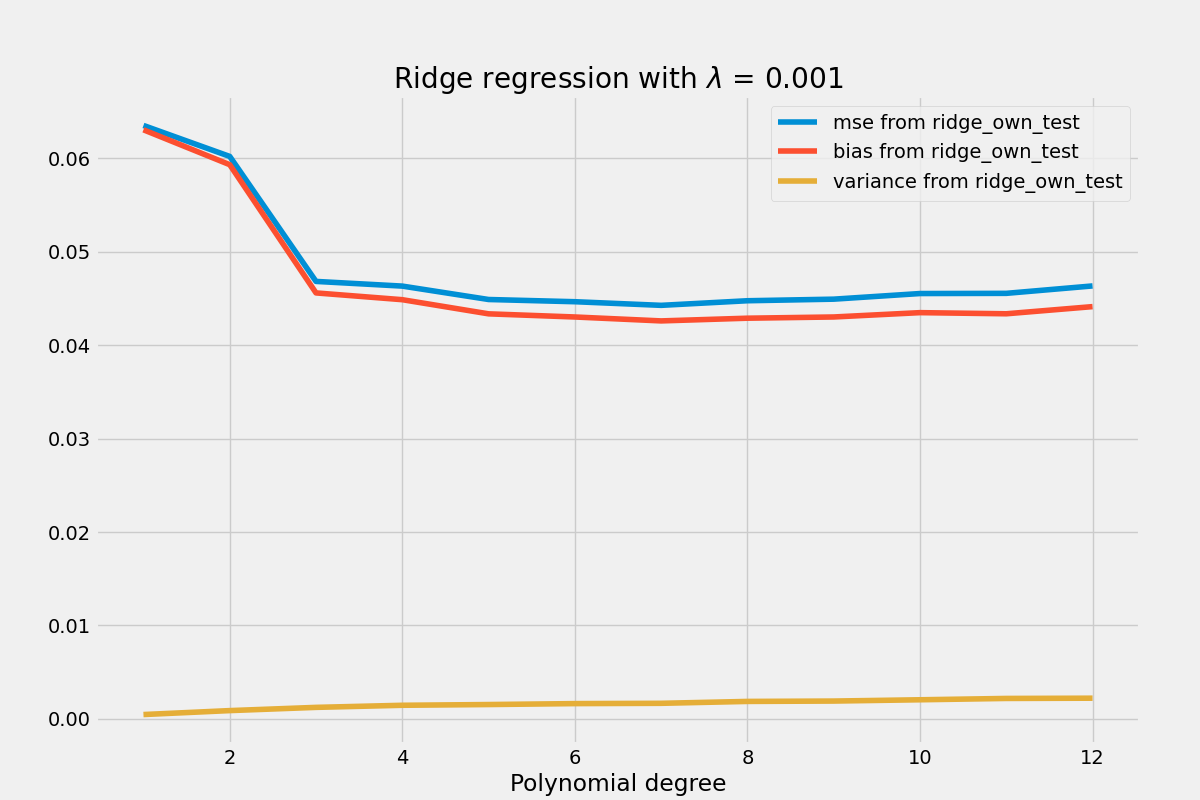
\includegraphics[width=0.8\textwidth]{Figures/e_ridge_bias_variance_lamb_0_001.png}
\end{figure}


\begin{figure}[H]
    \centering
    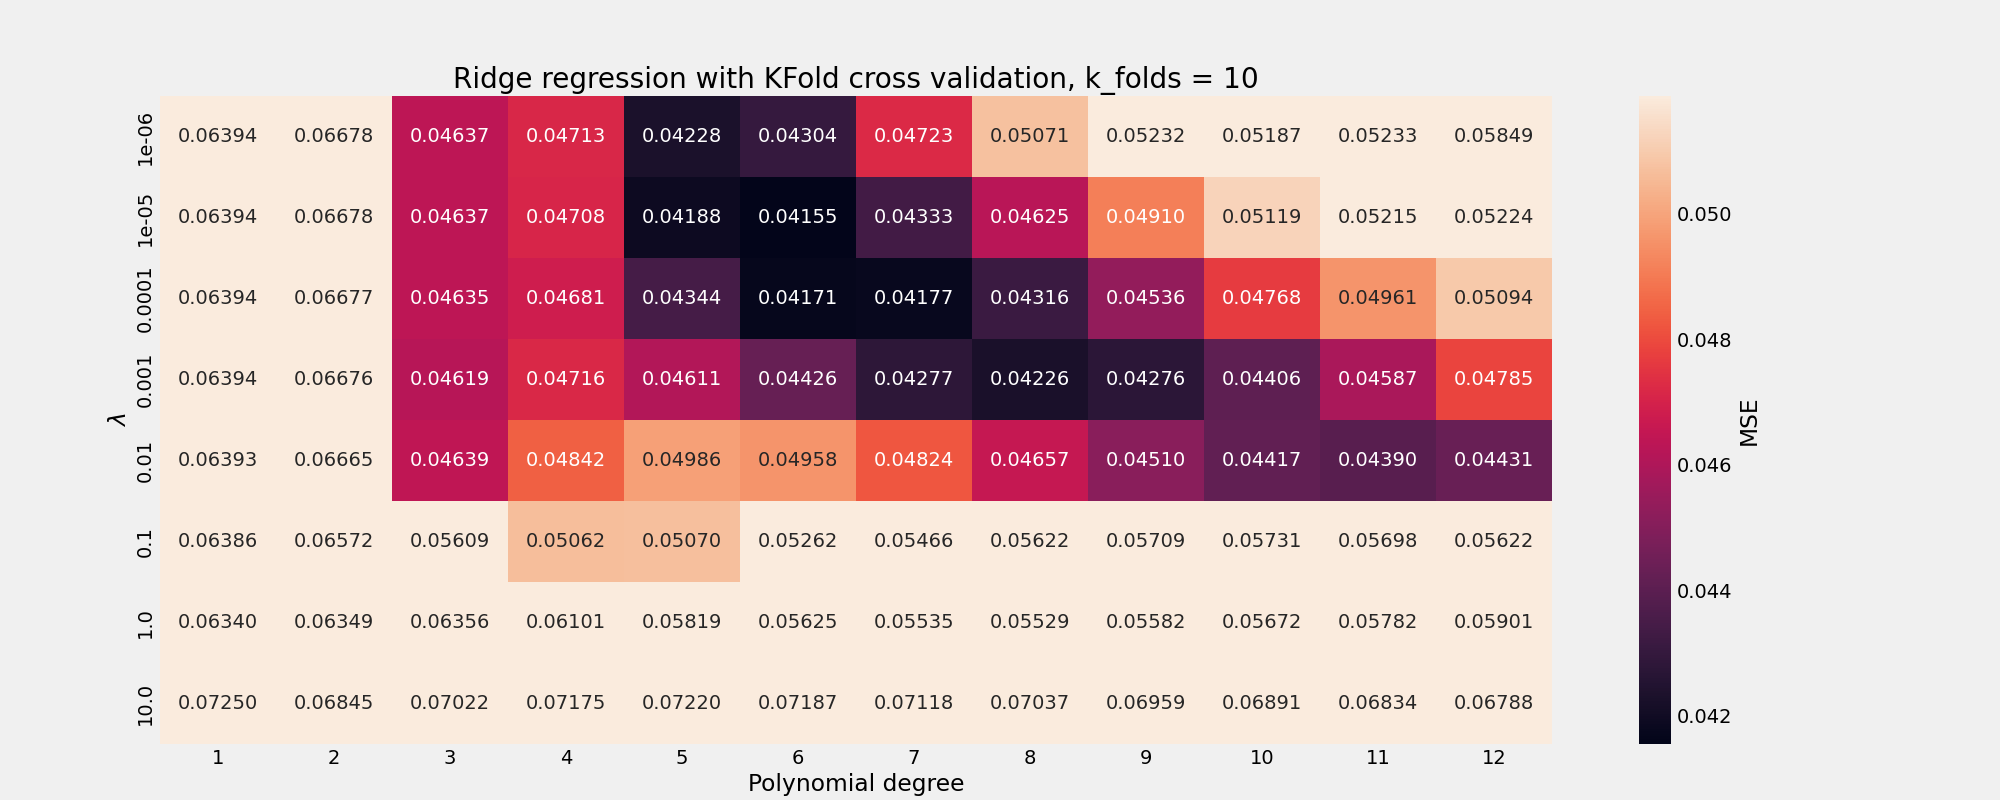
\includegraphics[width=0.8\textwidth]{Figures/e_ridge_kfold_n_10.png}
\end{figure}

%%%%%%%%%%%%%%% Part f %%%%%%%%%%%%%%%
% * Lasso regression
% * give a critical discussion of mse, ridge, lasso
% * Which model fits the data best 
% * bootstrap bias variance analysis of lasso
% * MSE analysis with kfold


\begin{figure}[H]
    \centering
    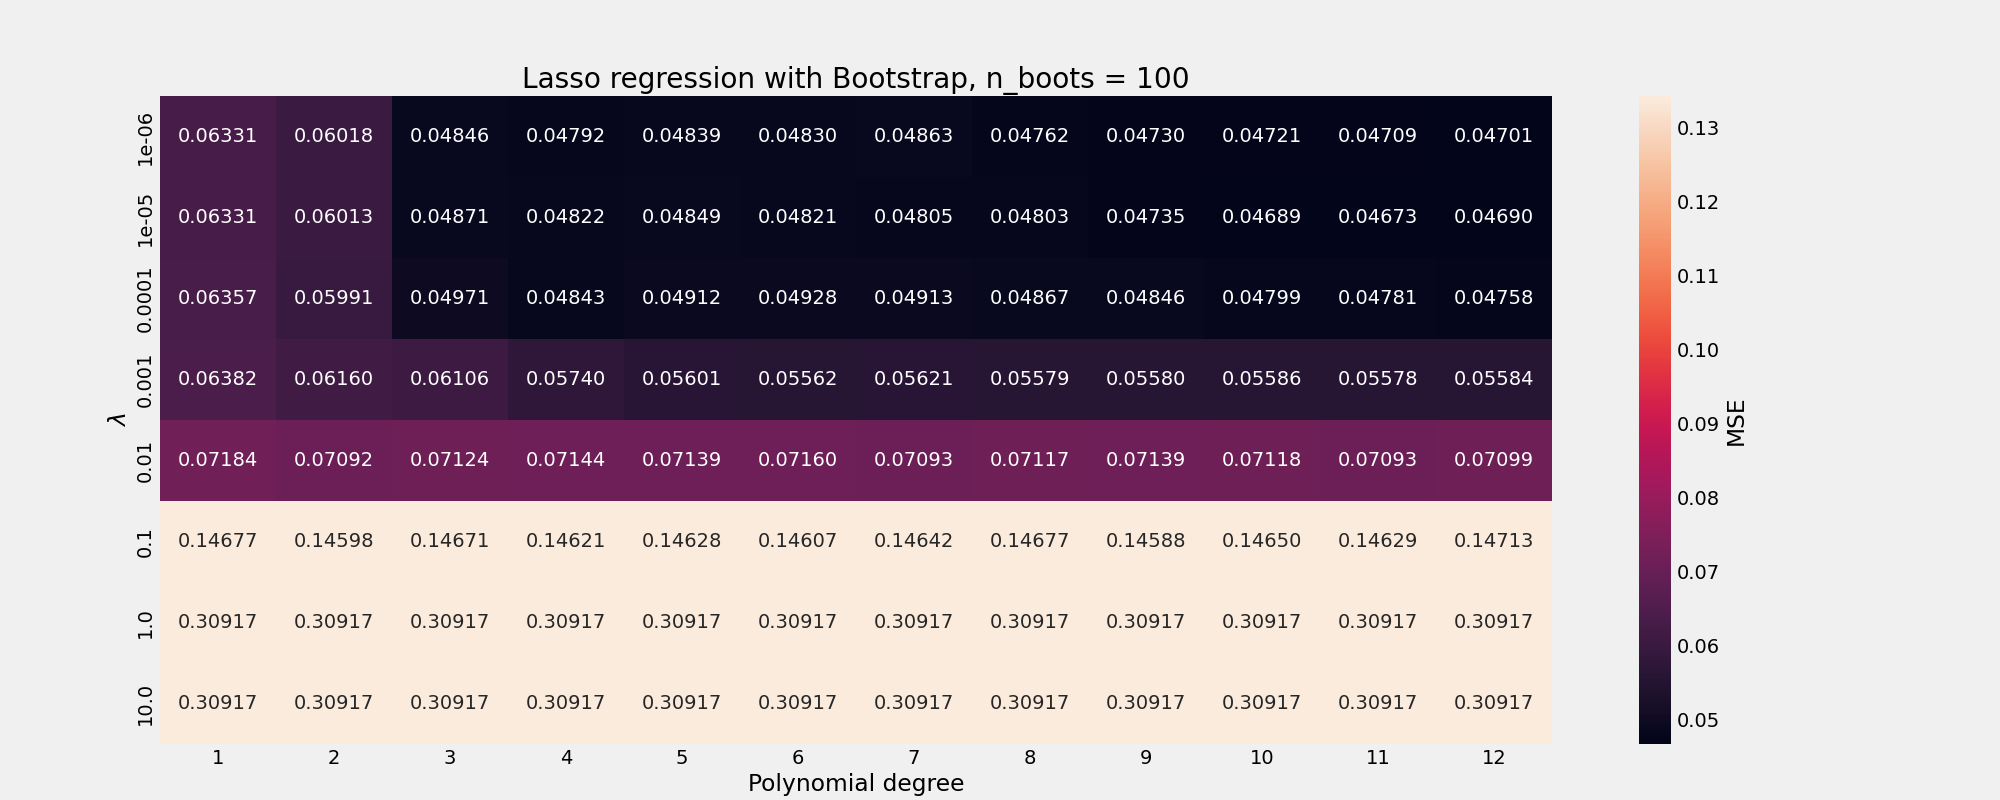
\includegraphics[width=0.8\textwidth]{Figures/f_lasso_bootstrap_n_100.png}
\end{figure}

\begin{figure}[H]
    \centering
    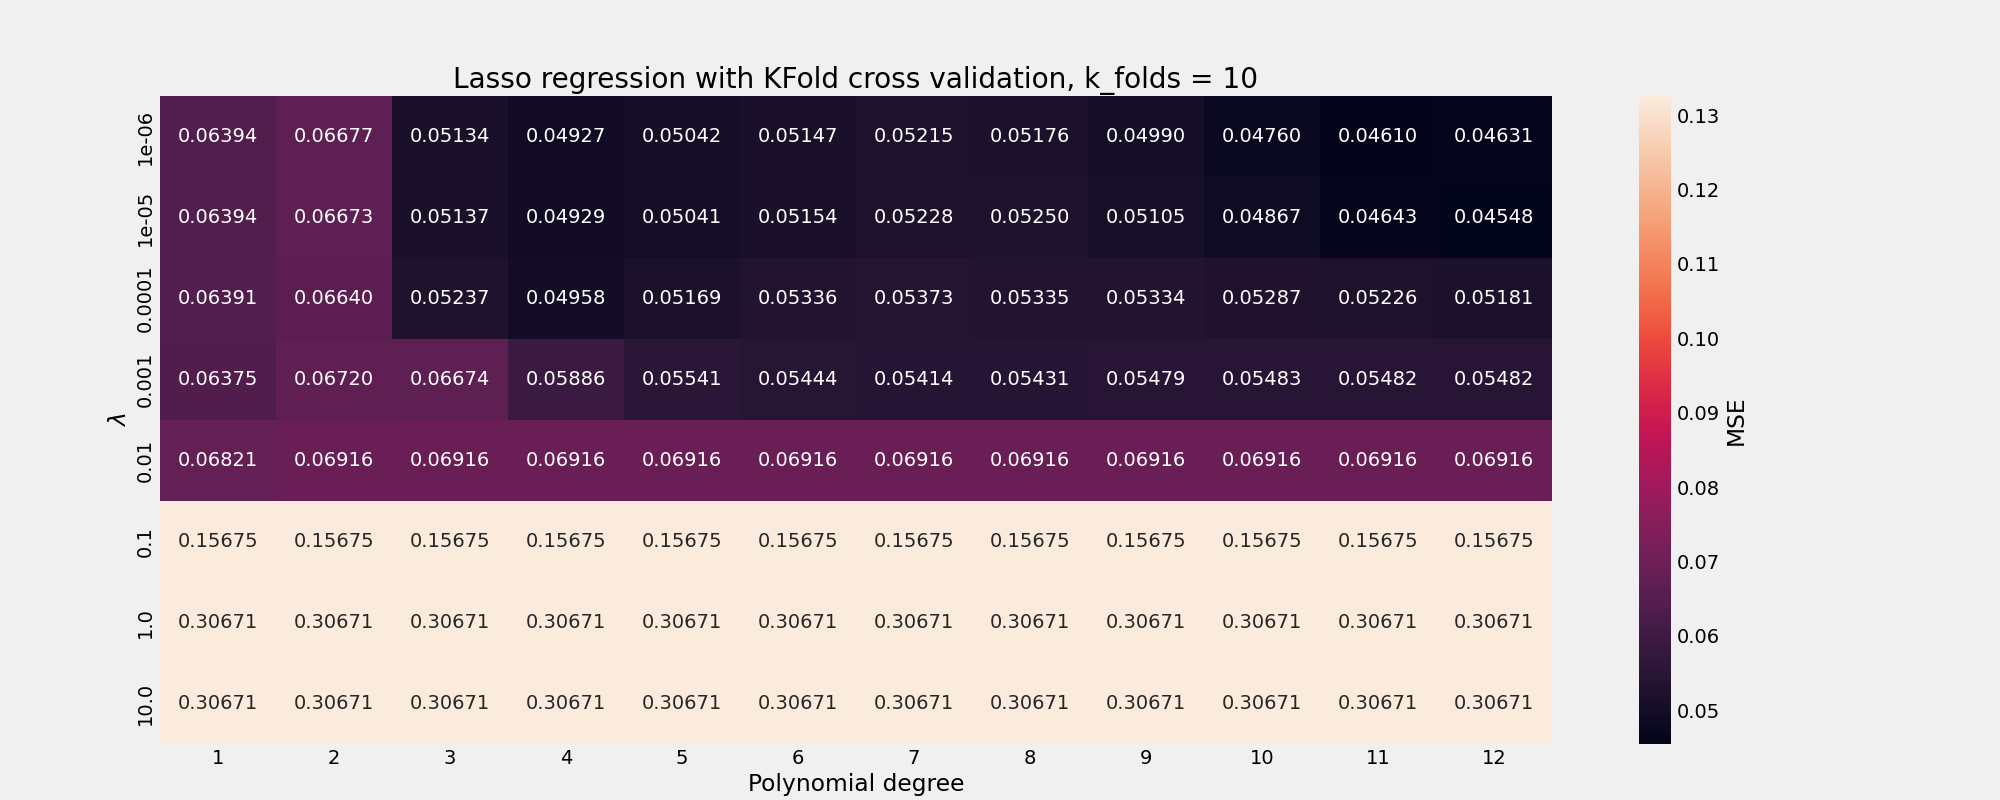
\includegraphics[width=0.8\textwidth]{Figures/f_lasso_kfold_n_10.png}
\end{figure}



% TODO: comparison of MSE for all methods
 
 %Maybe split results into two parts, Franke and Terrain data

%According to red line in report we want:
%On Franke-Function
%Subplot of MSE and R^2, test and training data, for OLS
%Subplot of MSE and R^2, test and training data, for Lasso
%Subplot of MSE and R^2, test and training data, for Ridge
%Comparrison of Regression methods
%Beta plot, but how to do this nicely, to show how beta values get large when polynomial degree increases.
%Resampling: bias-variance plot of bootstrap and cross-validation
%Study lambda dependence (correlation plot)

%On Terrain-data
%Subplot of MSE and R^2, test and training data, for OLS
%Subplot of MSE and R^2, test and training data, for Lasso
%Subplot of MSE and R^2, test and training data, for Ridge
%Comparrison of Regression methods
%Resampling: bias-variance plot of bootstrap and cross-validation
%Study lambda dependence (correlation plot)

%For critical discussion of centering/scaling, from lecture notes: "If our predictors represent different scales, then it is important to standardize the design matrix  by subtracting the mean of each column from the corresponding column and dividing the column with its standard deviation."




%%%%%%%%%%%%%%%%%%%%%%%%%%%%%%%%%%%%%%%%%%%%%
\subsection{Terrain data}


\begin{figure}
\centering
\begin{subfigure}{0.49\textwidth}
    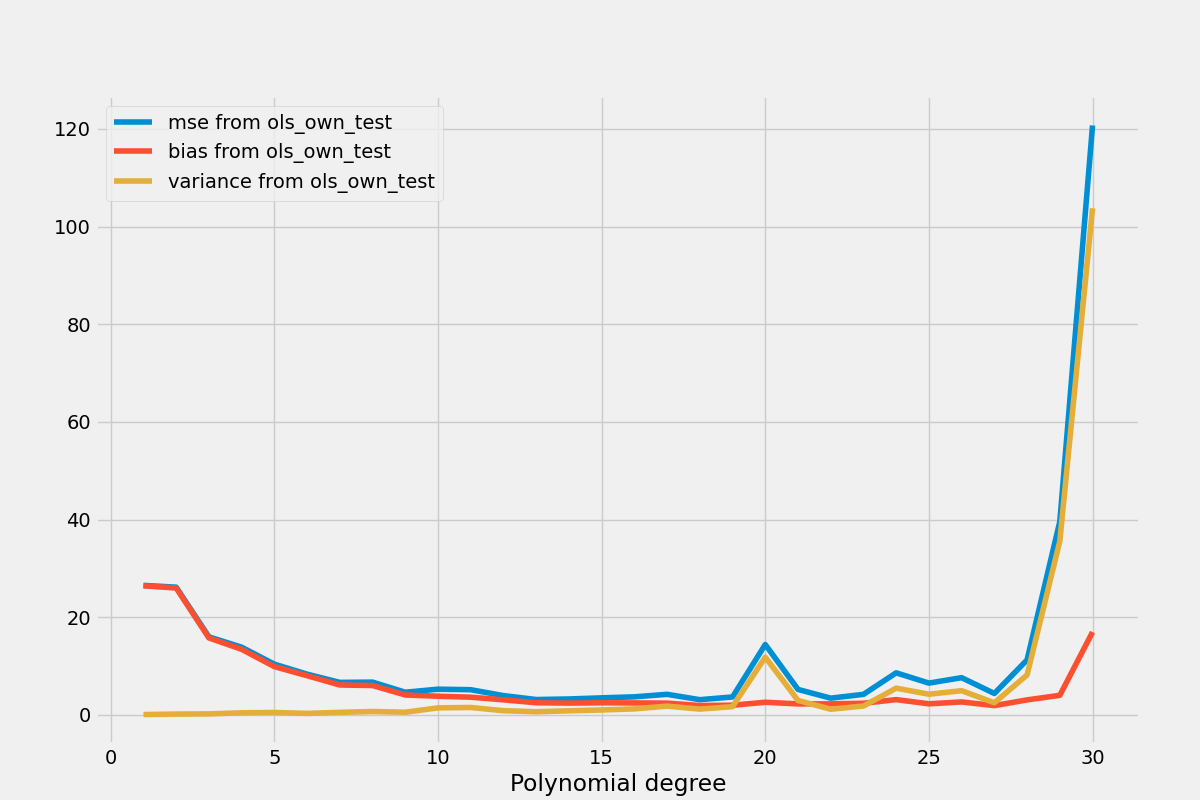
\includegraphics[width=\textwidth]{Figures/g_ols_bias_variance_boots_n_20.png}
    \caption{Bias, Variancse and MSE obtained with OLS and bootstrap re-sampling.
    20 re-samples was used to calculate the mean scores.}
    \label{fig:g_ols_bias_variance_boots}
\end{subfigure}
\hfill
\begin{subfigure}{0.49\textwidth}
    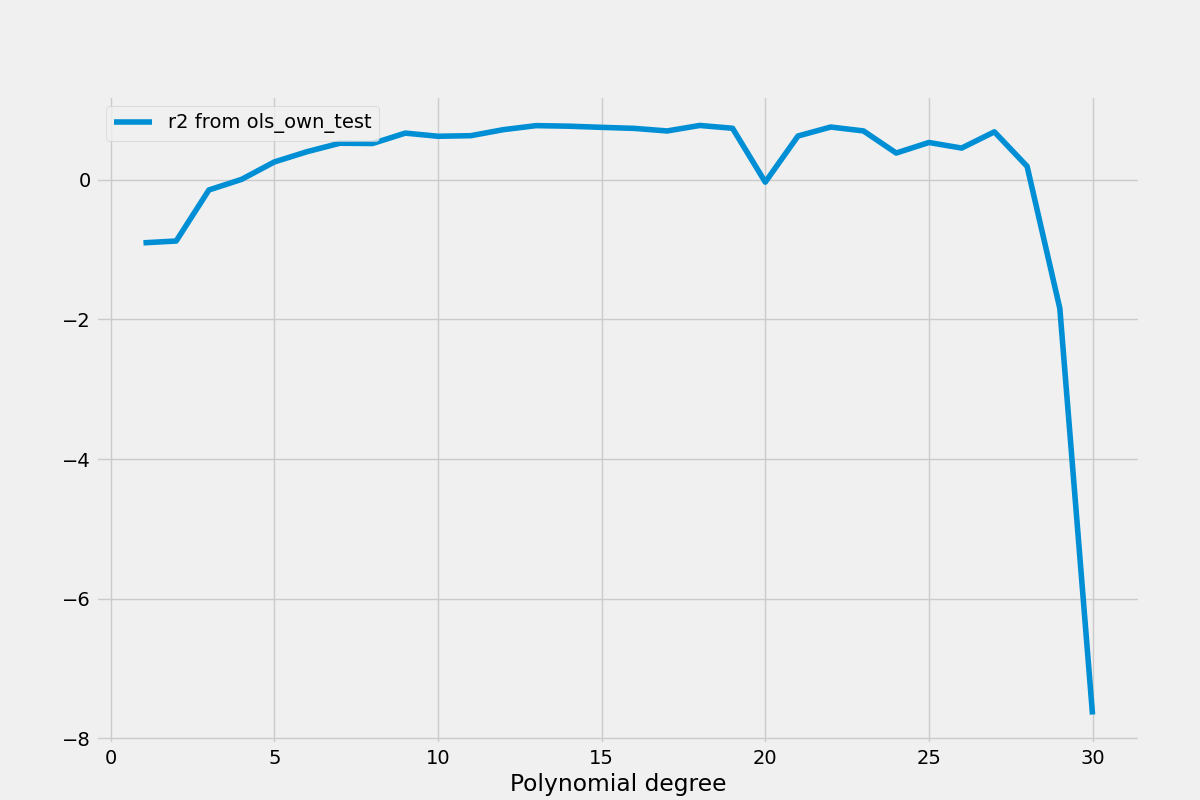
\includegraphics[width=\textwidth]{Figures/g_ols_r2_boots_n_20.png}
    \caption{R2 score obtained with OLS and bootstrap re-sampling.
    20 re-samples was used to calculate the mean R2 score.}
    \label{fig:g_ols_bias_variance_boots}
\end{subfigure}
\end{figure}


\begin{figure}[H]
    \centering
    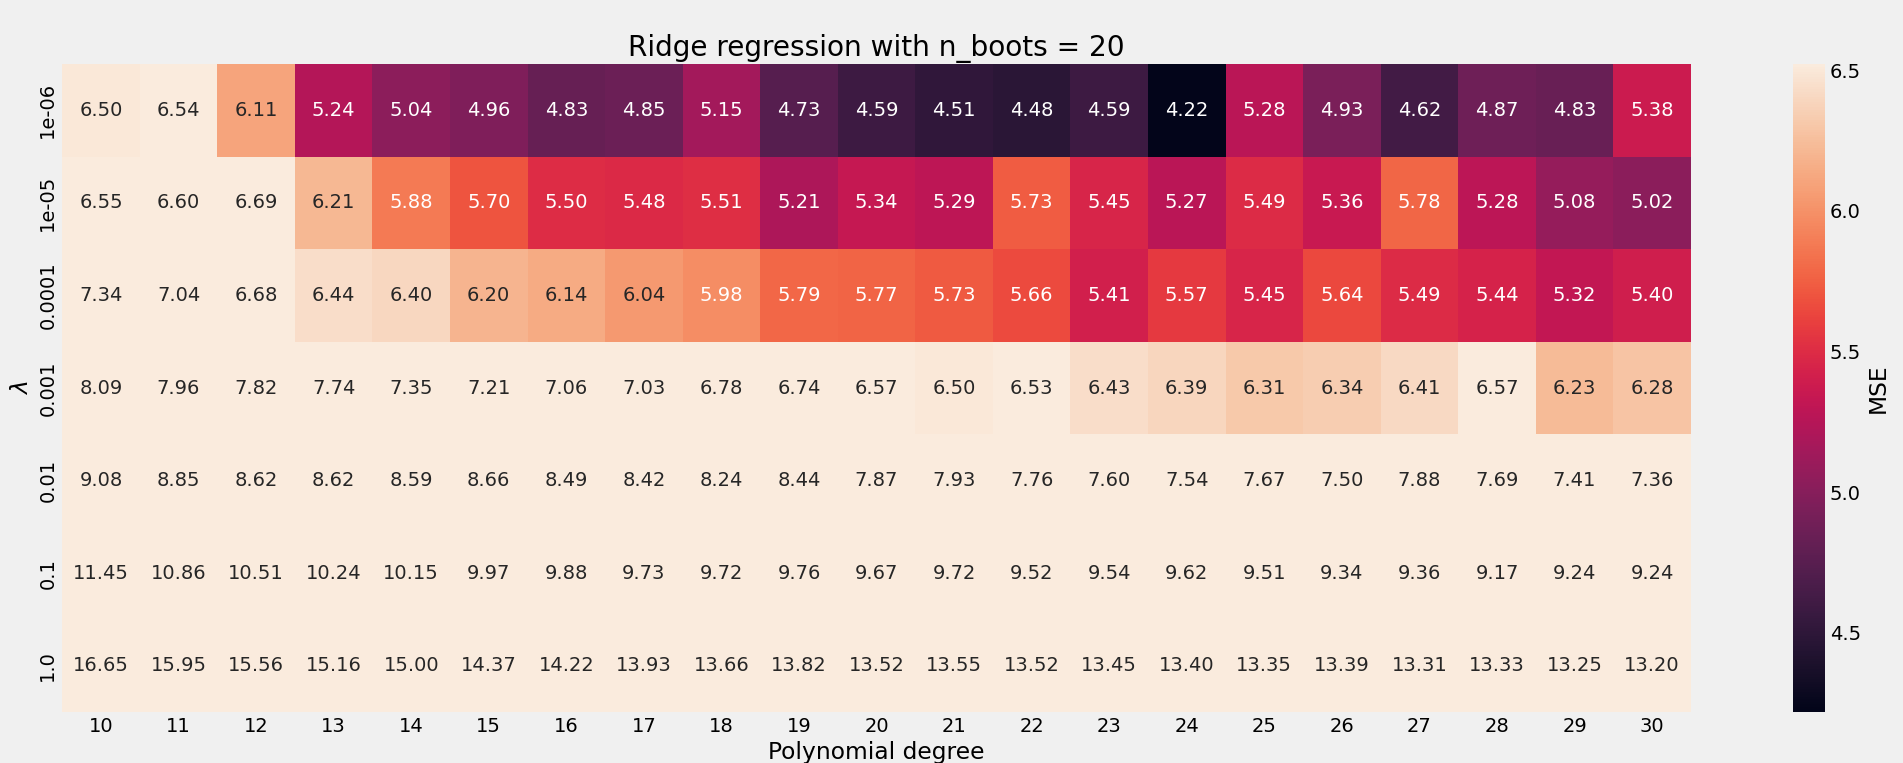
\includegraphics[width=\textwidth]{Figures/g_ridge_heatmap_boots_n_20.png}
    \caption{Heatmap of MSE scores obtained with Ridge regression and Bootstrap
    re-sampling, with 20 bootstrap re-sampling iterations.}  
    \label{fig:g_ridge_boost_heatmap}  
\end{figure}

\begin{figure}[H]
    \centering
    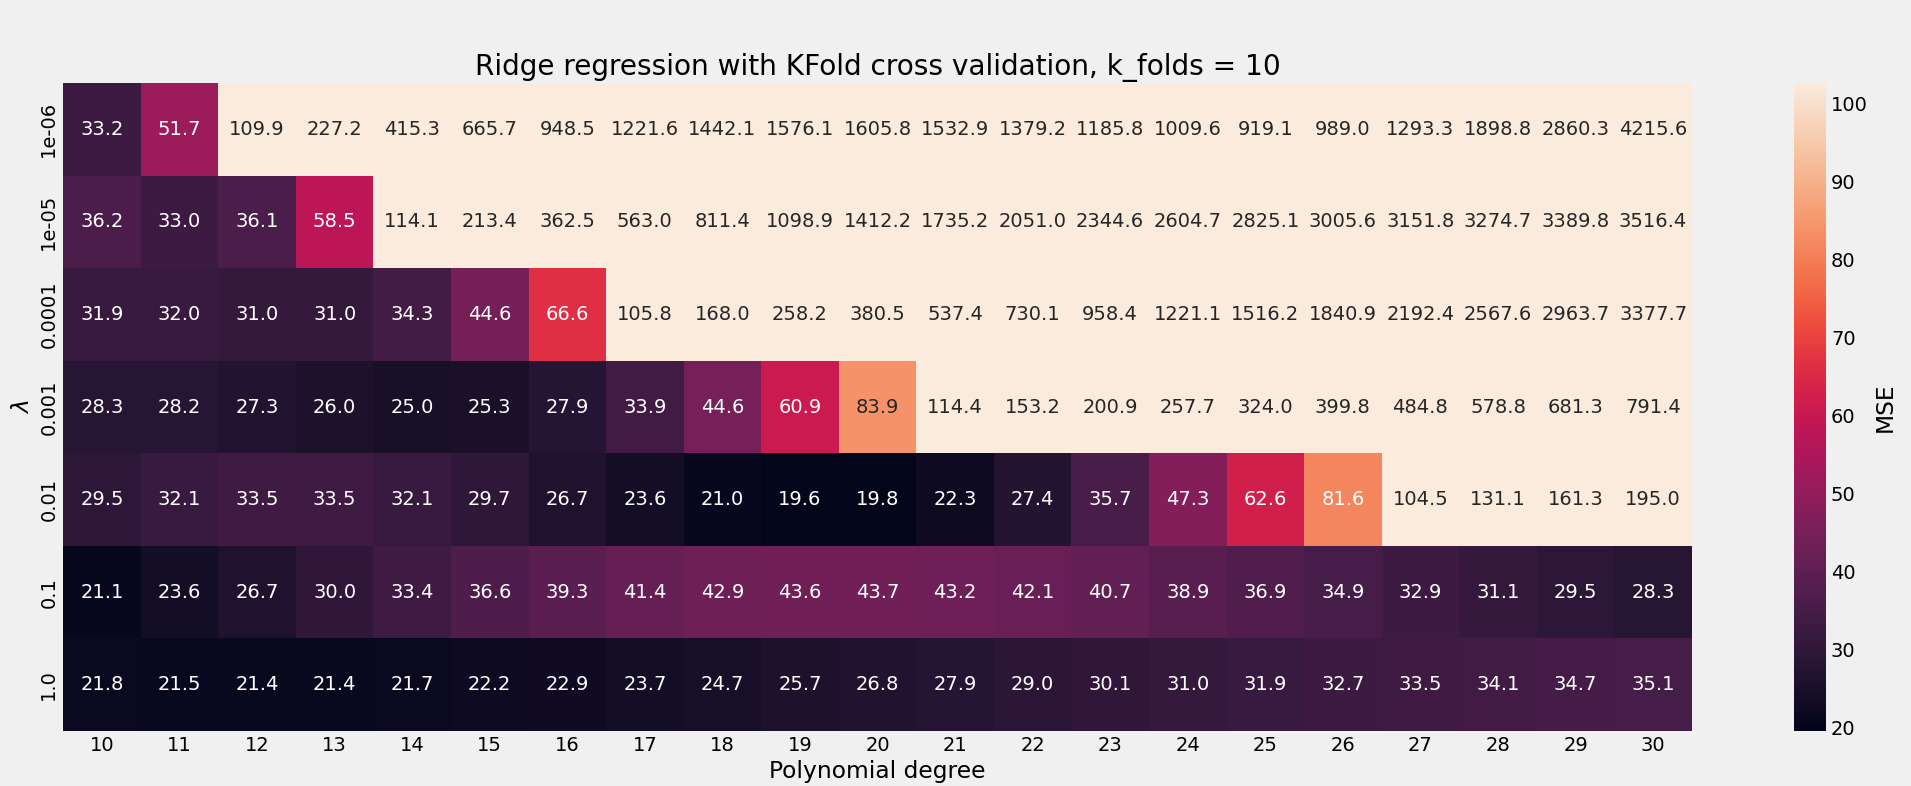
\includegraphics[width=\textwidth]{Figures/g_ridge_heatmap_kfold_n_10.png}
    \caption{Heatmap of MSE scores obtained with Ridge regression and K-fold
    re-sampling, with 10 splits.}  
    \label{fig:g_ridge_kfold_heatmap}  
\end{figure}

\begin{figure}[H]
    \centering
    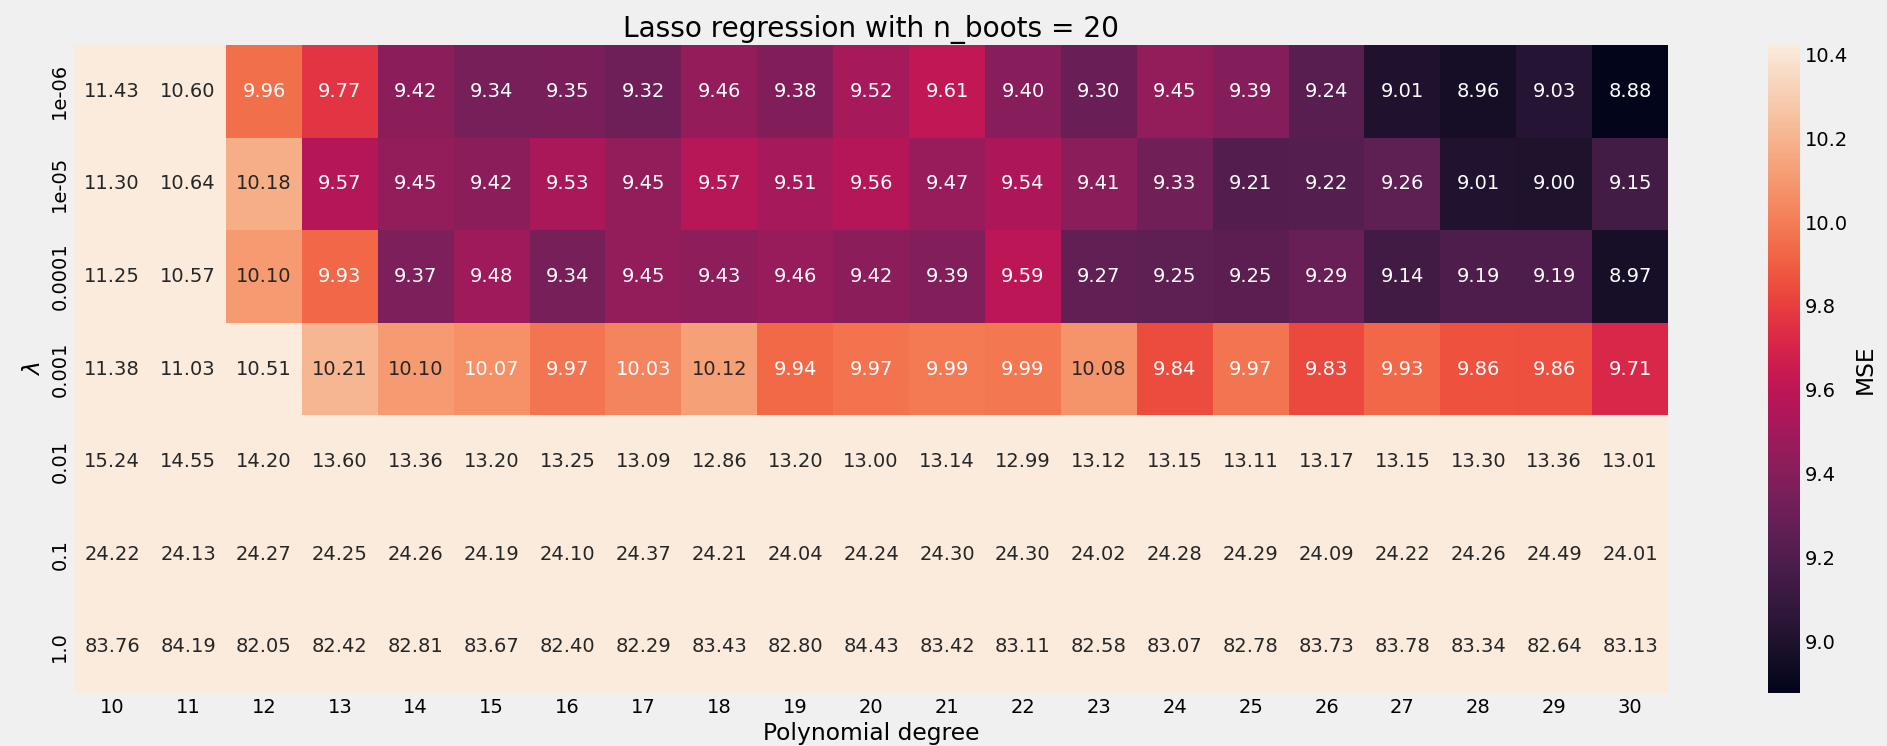
\includegraphics[width=\textwidth]{Figures/g_lasso_heatmap_boost_n_20.png}
    \caption{Heatmap of MSE scores obtained with lasso regression and Bootstrap
    re-sampling, with 20 re-samples.}  
    \label{fig:g_lasso_boots_heatmap}  
\end{figure}

\begin{figure}[H]
    \centering
    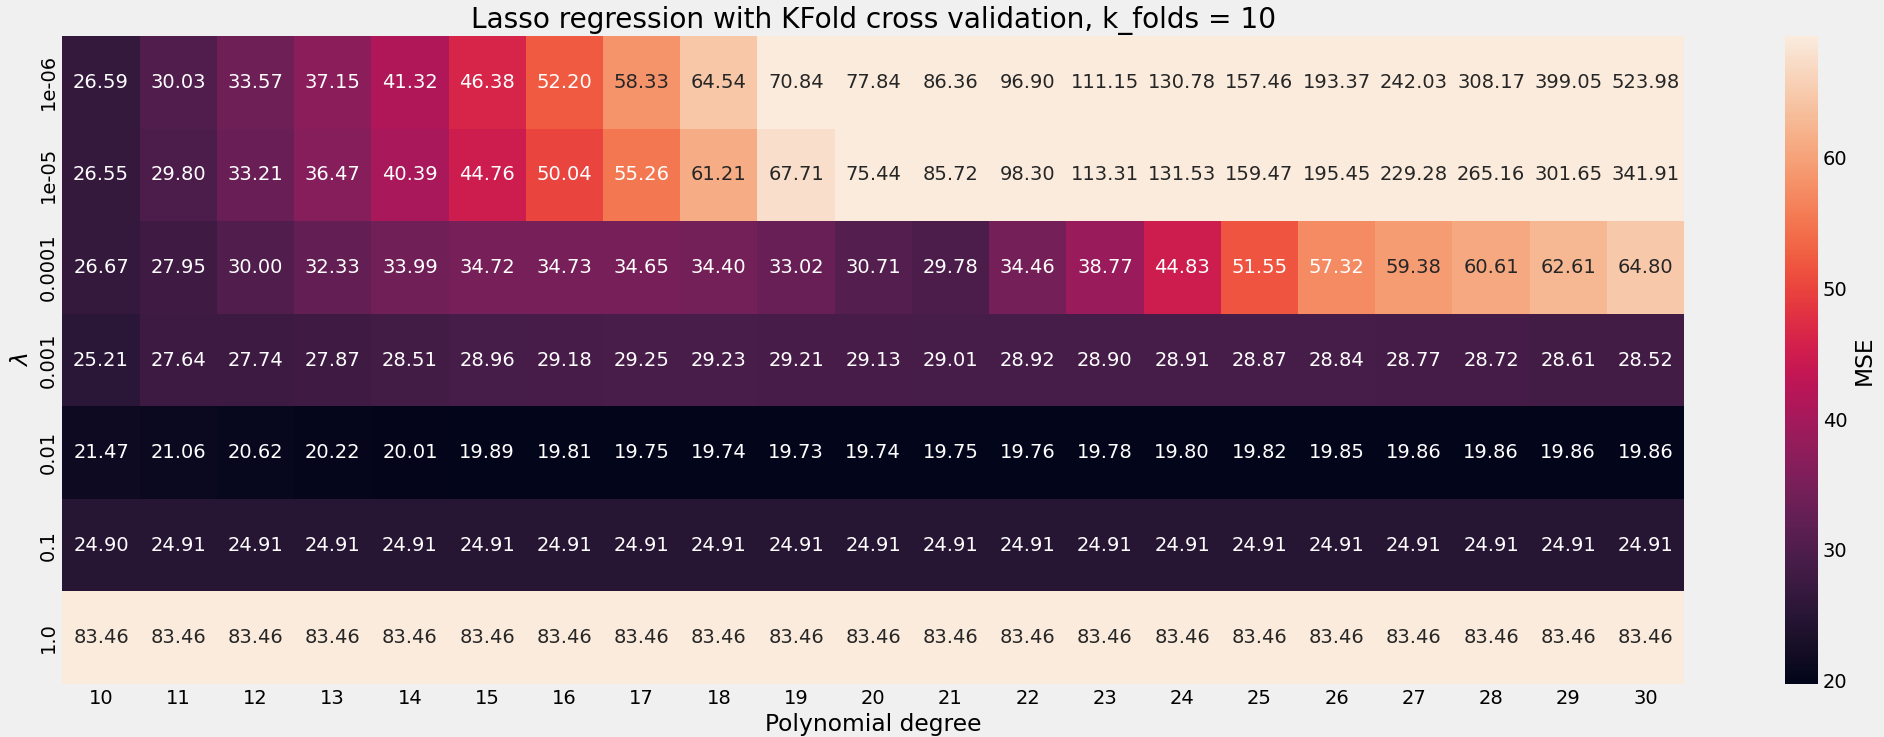
\includegraphics[width=\textwidth]{Figures/g_lasso_heatmap_kfold_n_10.png}
    \caption{Heatmap of MSE scores obtained with lasso regression and K-fold
    re-sampling, with 10 splits.}  
    \label{fig:g_lasso_boots_heatmap}  
\end{figure}



\begin{table}
    \centering
    \caption{Table of Best mean squared error (MSE) scores obtained with
        different re-sampling and regression
        methods. $\lambda $ is the best choice of regularization parameters for
        Ridge and Lasso regression. n refers to number of re-samples/splits used in
        Bootstrap and K-fold.}  
    \label{tab:mse_best} 
    \begin{tabular}{|c|c|c|c|c|}
        \hline
        Polynomial degree & $\lambda$ & Regression method & Re-sampling method & MSE \\
        \hline
                          18 &   &  OLS & Bootstrap (n=20) & 3.12\\
        \hline

                          24 & $10^{-6}$ &   Ridge & Bootstrap (n=20) & 4.22\\
        \hline

                          30 &  $10^{-6}$ & Lasso&  Bootstrap (n=20) & 8.88\\
        \hline

                          & & OLS & K-fold (n=10)& \\
        \hline

                          19 &  0.01 & Ridge & K-fold (n=10)& 19.6\\
        \hline

                          19 & 0.01 &  Lasso & K-fold (n=10)& 19.73\\
        \hline
    \end{tabular} 
\end{table}




\begin{figure}[H]
    \centering
    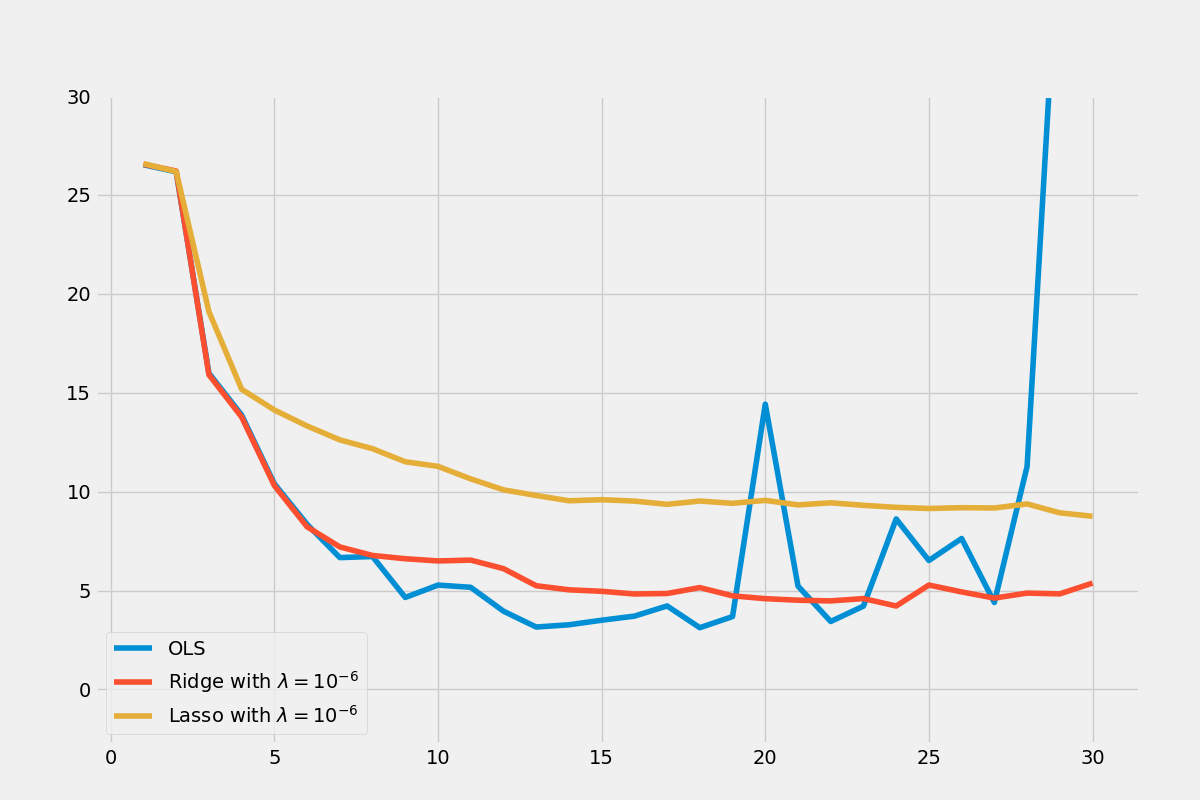
\includegraphics[width=0.8\textwidth]{Figures/g_ols_ridge_lasso_boots_n_20.png}
\end{figure}





